\chapter{Quantum information}
\label{ch:qinfo}

\buildson{quantum mechanics (Chapter~\ref{ch:qm})}

\chapterdek{Turning the weirdest features of quantum mechanics --- superposition, entanglement, the impossibility of copying --- into resources for computing, communication, and cryptography.}

\begin{prototype}
The entangled pair: two qubits in the Bell state $\tfrac{1}{\sqrt2}(\ket{00}+\ket{11})$. Measure either one and you get $0$ or $1$ at random; measure both and they always agree, along any axis, however far apart they are. Neither qubit has a state of its own. All the information is in the correlations.
\end{prototype}

For most of the twentieth century, the paradoxes of quantum mechanics --- superposition, entanglement, measurement --- were treated as philosophical puzzles to be explained away. Starting in the 1980s, physicists and computer scientists asked a different question: what can you \emph{do} with them? The answer turned out to be: quite a lot. Quantum information science treats quantum mechanics not as a strange theory of nature but as a new theory of information, with its own units, its own rules, and its own possibilities. It has produced provably secure cryptography, algorithms that would break most of today's encryption, and a global race to build quantum computers.

\section{Qubits}

A classical bit is $0$ or $1$. A \textbf{qubit} is a two-level quantum system (Chapter~\ref{ch:qm}) in a state
\[
  \ket\psi = \alpha\ket0 + \beta\ket1, \qquad\abs\alpha^2 + \abs\beta^2 = 1 .
\]
Since an overall phase has no physical meaning, a qubit state can be written as $\cos(\theta/2)\ket0 + e^{i\phi}\sin(\theta/2)\ket1$, a point on the surface of a sphere, the \textbf{Bloch sphere}: $\ket0$ at the north pole, $\ket1$ at the south, and superpositions everywhere else. The states $\ket\pm = (\ket0\pm\ket1)/\sqrt2$ sit on the equator. A qubit seems to contain a continuous infinity of information --- two real angles --- but measuring it yields a single bit, $0$ with probability $\abs\alpha^2$ or $1$ with probability $\abs\beta^2$, and destroys the superposition. The richness is in what can be done \emph{before} measurement.

Physically, a qubit can be an electron spin, the polarization of a photon, two energy levels of an atom or ion, or the lowest two states of a superconducting circuit.

\section{Many qubits and entanglement}

Two qubits have four basis states, $\ket{00},\ket{01},\ket{10},\ket{11}$, and their general state is a superposition of all four. $n$ qubits need $2^n$ complex amplitudes. Three hundred qubits require more amplitudes than there are atoms in the observable universe. This exponential growth is why quantum systems are so hard to simulate on classical computers --- and why Richard Feynman suggested in 1981 that we simulate them with quantum computers instead.

Most of these states are \emph{entangled}: they cannot be written as a product of single-qubit states. The four \textbf{Bell states},
\[
  \ket{\Phi^\pm} = \frac{\ket{00}\pm\ket{11}}{\sqrt2},\qquad \ket{\Psi^\pm} = \frac{\ket{01}\pm\ket{10}}{\sqrt2},
\]
form a basis of maximally entangled states. Measure the first qubit of $\ket{\Phi^+}$ and you get $0$ or $1$ at random; the second then always gives the same. This is not like a pair of gloves, one left and one right, separated in boxes: as Bell showed (\S\ref{sec:chsh}), no assignment of pre-existing values reproduces the correlations measured along \emph{different} axes.

\section{You cannot copy a qubit}

\begin{theorem}[No-cloning]
There is no physical process that takes an unknown quantum state $\ket\psi$ and produces two copies, $\ket\psi\ket\psi$.
\end{theorem}
The proof is two lines, and uses only linearity (Problem~\ref{prob:noclone}). Suppose a machine copies $\ket0$ and $\ket1$ correctly. Then by linearity it must turn $\alpha\ket0+\beta\ket1$ into $\alpha\ket{00}+\beta\ket{11}$ --- an entangled state, not two copies. No-cloning is why entanglement cannot transmit signals faster than light (Bob cannot make many copies of his qubit to find out what Alice measured), and why quantum cryptography is secure (an eavesdropper cannot copy the key).

\section{Gates and circuits}

A quantum computation is a sequence of \emph{gates}: unitary operations (Chapter~\ref{ch:qm}) acting on one or two qubits at a time. Because they are unitary, quantum gates are reversible. Important single-qubit gates include the Pauli gates $X$ (bit flip, $\ket0\leftrightarrow\ket1$) and $Z$ (phase flip, $\ket1\to-\ket1$), and the \textbf{Hadamard} gate
\[
  H = \frac{1}{\sqrt2}\begin{pmatrix}1&1\\1&-1\end{pmatrix},\qquad H\ket0 = \ket+,\quad H\ket1 = \ket- ,
\]
which turns a definite bit into an equal superposition and back again. The essential two-qubit gate is the \textbf{controlled-NOT} (CNOT), which flips the second qubit if and only if the first is $1$. A Hadamard followed by a CNOT turns two unentangled qubits into a Bell state:

\begin{center}
\begin{tikzpicture}[line width=0.8pt]
  \draw (0,0) node[left]{$\ket0$} -- (4.2,0);
  \draw (0,-1.1) node[left]{$\ket0$} -- (4.2,-1.1);
  \node[draw,fill=white,minimum size=0.7cm] at (1.2,0) {$H$};
  \draw (2.7,0) -- (2.7,-1.3);
  \fill (2.7,0) circle (2.6pt);
  \draw[fill=white] (2.7,-1.1) circle (0.2);
  \draw (2.5,-1.1) -- (2.9,-1.1);
  \draw (2.7,-0.9) -- (2.7,-1.3);
  \node[right] at (4.3,-0.55) {$\dfrac{\ket{00}+\ket{11}}{\sqrt2}$};
\end{tikzpicture}
\end{center}

A small set of gates --- for example $H$, CNOT, and a rotation by $\pi/8$ --- is \emph{universal}: any unitary operation on any number of qubits can be approximated by a circuit built from them.

\section{Protocols}

\textbf{Superdense coding.} Alice and Bob share a Bell pair. By applying one of four operations ($I$, $X$, $Z$, or $XZ$) to her qubit alone, Alice can turn the pair into any of the four Bell states. She sends her qubit to Bob, who measures both in the Bell basis and learns which. One qubit has carried two classical bits.

\textbf{Teleportation.} Alice holds an unknown qubit $\ket\psi$ and shares a Bell pair with Bob. She makes a joint Bell measurement on $\ket\psi$ and her half of the pair, and phones Bob the result: two classical bits. Bob applies a correction ($I$, $X$, $Z$, or $XZ$) to his half, which is now exactly $\ket\psi$ (Problem~\ref{prob:teleport}). The original is destroyed in the process, as no-cloning demands; nothing travels faster than light, since Bob must wait for the phone call. Teleportation is routine in laboratories and has been done between the ground and a satellite over $1200\un{km}$.

\textbf{Quantum key distribution.} In the BB84 protocol (Bennett and Brassard, 1984), Alice sends single photons, each randomly prepared in one of two bases ($\ket0,\ket1$ or $\ket+,\ket-$). Bob measures each in a randomly chosen basis. Afterwards they announce publicly which bases they used --- not the results --- and keep only the bits where the bases matched, giving a shared secret key. An eavesdropper who measures the photons must guess the basis, and half the time guesses wrong, disturbing the state and introducing errors at a rate of $25\%$ in the kept bits (Problem~\ref{prob:bb84}). Alice and Bob detect her by comparing a sample. The security rests on the laws of physics, not on the presumed difficulty of a mathematical problem.

\section{Bell's inequality, sharpened}
\label{sec:chsh}

Suppose Alice can measure one of two quantities $A$ or $A'$, and Bob one of $B$ or $B'$, each with outcomes $\pm1$. If the outcomes are determined in advance by some local hidden variables, then for every run, $A(B+B') + A'(B-B')$ equals $\pm2$ (one bracket is zero and the other is $\pm2$). Averaging gives the \textbf{CHSH inequality}:
\[
  S = \abs{\expval{AB} + \expval{AB'} + \expval{A'B} - \expval{A'B'}}\le 2.
\]
For a Bell pair, with spin measurements along suitably chosen axes, quantum mechanics predicts $S = 2\sqrt2\approx2.83$ (Problem~\ref{prob:chsh}). Experiments find $2.8$. No local hidden variable theory can reproduce the predictions of quantum mechanics. In 2015 three groups closed the remaining loopholes, and Aspect, Clauser, and Zeilinger shared the 2022 Nobel Prize for the decades of experiments that led there. Remarkably, quantum mechanics itself cannot exceed $2\sqrt2$ (\emph{Tsirelson's bound}, Problem~\ref{prob:tsirelson}), though logic alone would allow $S$ up to $4$. Why nature stops exactly at $2\sqrt2$ is a deep question.

\section{Quantum algorithms}

A quantum computer is not a faster classical computer. It cannot simply try all answers at once and read out the right one: measurement returns a single random outcome. The trick of every quantum algorithm is to arrange \emph{interference} so that amplitudes for wrong answers cancel and amplitudes for right answers add up.

\textbf{Deutsch's problem.} Given a black box computing $f:\{0,1\}\to\{0,1\}$, decide whether $f$ is constant or balanced. Classically, you must query it twice. Quantumly, once suffices, by querying a superposition and letting the two branches interfere (Problem~\ref{prob:deutsch}). It is a toy, but the first proof that quantum computers can do something classical ones cannot.

\textbf{Grover's search.} To find a marked item among $N$ unsorted items, a classical computer needs about $N/2$ guesses. Grover's algorithm (1996) needs only about $\tfrac\pi4\sqrt N$, by repeatedly reflecting the state about the marked item and about the average, rotating it step by step toward the answer. A quadratic speedup, applicable to any search problem.

\textbf{Shor's algorithm.} In 1994 Peter Shor showed that a quantum computer could factor large numbers exponentially faster than any known classical method. Factoring reduces to finding the period of a function, and a quantum computer can find periods efficiently using the \emph{quantum Fourier transform}, which applies the Fourier transform (Chapter~\ref{ch:math}) to $2^n$ amplitudes with only about $n^2$ gates. The security of the RSA encryption that protects most internet traffic rests on factoring being hard. Shor's algorithm launched the field, and governments are already replacing RSA with ``post-quantum'' cryptography in anticipation.

\textbf{Quantum simulation.} Feynman's original motivation remains perhaps the most important application: simulating molecules (Chapter~\ref{ch:chem}), materials (Chapter~\ref{ch:condmat}), and nuclear matter, whose quantum states are exponentially hard to represent classically.

\section{Decoherence and mixed states}

Real qubits are fragile. Their interactions with the environment --- stray fields, vibrations, a single photon --- entangle them with the outside world, and the delicate phase relationships that make a superposition quantum leak away. This is \emph{decoherence} (Chapter~\ref{ch:qm}).

To describe a qubit that may be entangled with things we are not tracking, we use the \emph{density matrix} $\rho$. A pure state $\ket\psi$ has $\rho = \ket\psi\bra\psi$. A random mixture of states $\ket{\psi_i}$ with probabilities $p_i$ has $\rho = \sum_ip_i\ket{\psi_i}\bra{\psi_i}$. The state $\ket+$ and a 50/50 coin-flip mixture of $\ket0$ and $\ket1$ give identical statistics when measured in the $\{\ket0,\ket1\}$ basis, but very different ones in the $\{\ket+,\ket-\}$ basis; their density matrices differ in the off-diagonal elements, the \emph{coherences}. Decoherence is the decay of those off-diagonal elements. The time it takes, $T_2$, ranges from microseconds for superconducting qubits to many seconds for trapped ions.

\section{Quantum error correction}

Classical computers fight errors by copying: store each bit three times and take a majority vote. Quantum computers cannot copy (no-cloning), cannot look at their data without destroying it, and suffer continuous rather than discrete errors. For a while it seemed quantum computing was doomed. Then in 1995 Shor showed that quantum error correction is possible after all.

The idea, in the simplest \emph{bit-flip code}, is to encode one logical qubit as $\alpha\ket{000}+\beta\ket{111}$ --- entangled, not copied. If one physical qubit flips, measuring the \emph{parities} $Z_1Z_2$ and $Z_2Z_3$ reveals which one, without revealing anything about $\alpha$ and $\beta$, and the error can be undone (Problem~\ref{prob:bitflip}). More elaborate codes protect against all errors. The \textbf{threshold theorem} says that if each physical gate fails with probability below some threshold (about $1\%$ for the leading \emph{surface code}), then arbitrarily long quantum computations are possible by adding more physical qubits per logical one. In 2023 and 2024, experiments demonstrated logical qubits whose error rates \emph{fall} as the code is made bigger --- crossing the threshold for the first time.

\section{Building quantum computers}

Several physical platforms are in a tight race:
\begin{itemize}[itemsep=3pt]
  \item \textbf{Superconducting circuits}: tiny loops of superconductor interrupted by Josephson junctions (Chapter~\ref{ch:condmat}), cooled to $10\un{mK}$, behaving as artificial atoms. Fast gates, short coherence, fabricated like computer chips.
  \item \textbf{Trapped ions}: individual atoms held in electromagnetic traps and manipulated with lasers (Chapter~\ref{ch:amo}). Superb fidelity and long coherence, but slower gates.
  \item \textbf{Neutral atoms} held in arrays of optical tweezers and entangled via highly excited Rydberg states; hundreds to thousands of qubits.
  \item \textbf{Photons}, natural carriers of quantum information over long distances; and \textbf{spins} in silicon, which could ride on existing semiconductor manufacturing.
\end{itemize}
Today's machines have hundreds to a few thousand physical qubits and the first handfuls of error-corrected logical qubits. Useful fault-tolerant quantum computing will require millions of physical qubits, and its arrival date is an open question. Meanwhile, quantum \emph{sensors} --- atomic clocks, magnetometers, interferometers --- already outperform classical ones, and quantum networks are being built.

\section{Problems}

\begin{problems}
\prob{1}\core Locate the states $\ket0$, $\ket1$, $\ket+$, $\ket-$, and $(\ket0+i\ket1)/\sqrt2$ on the Bloch sphere. Show that $H^2 = I$, and describe $H$ geometrically as a rotation of the Bloch sphere.

\prob{1} Two qubits are in the state $\ket{\Phi^+}$. Show that measuring both in the $\{\ket0,\ket1\}$ basis always gives equal results. Rewrite $\ket{\Phi^+}$ in the $\{\ket+,\ket-\}$ basis and show that the results also always agree there.

\prob{1} How many complex amplitudes describe $50$ qubits? If each is stored as $16$ bytes, how much memory would a classical simulation need? What about $300$ qubits?

\prob{2}\core \label{prob:noclone} Prove the no-cloning theorem: assume a unitary $U$ satisfies $U\ket\psi\ket0 = \ket\psi\ket\psi$ for all $\ket\psi$, take the inner product of this equation for two states $\ket\psi$ and $\ket\phi$, and show that $\braket\psi\phi$ must be $0$ or $1$.

\prob{2} Verify superdense coding: show that applying $I$, $X$, $Z$, and $XZ$ to the first qubit of $\ket{\Phi^+}$ produces the four distinct Bell states.

\prob{2}\core \label{prob:teleport} \emph{(Teleportation.)} Write the three-qubit state $(\alpha\ket0+\beta\ket1)\otimes\ket{\Phi^+}$, where Alice holds the first two qubits and Bob the third. Rewrite Alice's two qubits in the Bell basis and show that the total state is
\[
  \tfrac12\Big[\ket{\Phi^+}(\alpha\ket0+\beta\ket1) + \ket{\Phi^-}(\alpha\ket0-\beta\ket1) + \ket{\Psi^+}(\beta\ket0+\alpha\ket1) + \ket{\Psi^-}(\alpha\ket1-\beta\ket0)\Big].
\]
For each of Alice's four outcomes, what correction must Bob apply?

\prob{2} Run Grover's algorithm by hand for $N=4$ items: start in the uniform superposition, flip the sign of the marked item's amplitude, then reflect all amplitudes about their average. Show that after one iteration the marked item has probability exactly $1$.

\prob{2}\core \label{prob:chsh} For the singlet state, the correlation between spin measurements along unit vectors $\vu a$ and $\vu b$ is $\expval{AB} = -\vu a\cdot\vu b$. Choose $\vu a$, $\vu a'$, $\vu b$, $\vu b'$ in a plane at angles $0^\circ$, $90^\circ$, $45^\circ$, and $-45^\circ$, and show that $S = 2\sqrt2$. (Try $\vu b'$ at $135^\circ$ instead: what goes wrong?)

\prob{2} Write the density matrices for the pure state $\ket+$ and for an equal mixture of $\ket0$ and $\ket1$. Show that they give the same statistics for $Z$-measurements but different ones for $X$-measurements, and that $\tr\rho^2$ is $1$ for the first and $\tfrac12$ for the second.

\prob{2} \label{prob:bb84} In BB84, an eavesdropper intercepts every photon, measures it in a randomly chosen basis, and resends what she found. Show that in the bits Alice and Bob keep, the error rate is $25\%$.

\prob{3}\core \label{prob:bitflip} \emph{(The three-qubit code.)} A logical qubit is encoded as $\alpha\ket{000}+\beta\ket{111}$, and then one of the three qubits may be flipped by $X$. Show that measuring the observables $Z_1Z_2$ and $Z_2Z_3$ (each $\pm1$) identifies which qubit, if any, was flipped, and that the measurement leaves $\alpha$ and $\beta$ untouched. Why does this code fail if two qubits flip, and why doesn't it protect against phase errors?

\prob{3} \label{prob:deutsch} \emph{(Deutsch's algorithm.)} A black box implements $\ket x\ket y\mapsto\ket x\ket{y\oplus f(x)}$. Prepare $\ket0\ket1$, apply $H$ to both qubits, apply the black box once, then apply $H$ to the first qubit and measure it. Show that the result is $0$ if $f$ is constant and $1$ if it is balanced.
\hint{Show that the box acting on $\ket x\ket-$ gives $(-1)^{f(x)}\ket x\ket-$: the function's value has been ``kicked back'' into a phase.}

\prob{3} \label{prob:tsirelson} \emph{(Tsirelson's bound.)} Let $A, A', B, B'$ be observables with eigenvalues $\pm1$, so $A^2 = B^2 = 1$, with Alice's operators commuting with Bob's. Define $C = AB + AB' + A'B - A'B'$. Show that $C^2 = 4 - [A,A'][B,B']$, and use $\norm{[A,A']}\le2$ to conclude that $\abs{\expval C}\le2\sqrt2$.
\end{problems}

\begin{reading}
\rd{Nielsen and Chuang, \emph{Quantum Computation and Quantum Information}}{The field's standard textbook, comprehensive and still the reference.}
\rd{N.\ David Mermin, \emph{Quantum Computer Science: An Introduction}}{A short, elegant introduction for those who know some linear algebra but no quantum mechanics.}
\rd{John Preskill, lecture notes for Caltech Ph219}{Deep, clear, and free online.}
\rd{Scott Aaronson, \emph{Quantum Computing Since Democritus}}{A witty tour of quantum computing and complexity theory.}
\end{reading}
